\documentclass{standalone}
\usepackage{tikz}
\usepackage{ctex,siunitx}
\setCJKmainfont{Noto Serif CJK SC}
\usepackage{tkz-euclide}
\usepackage{amsmath}
\usepackage{wasysym}
\usetikzlibrary{patterns, calc}
\usetikzlibrary {decorations.pathmorphing, decorations.pathreplacing, decorations.shapes,}
\begin{document}
\small
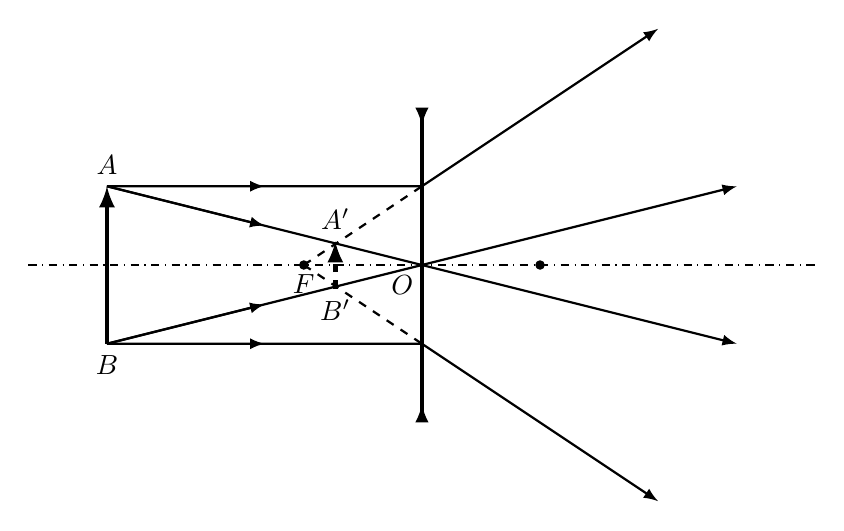
\begin{tikzpicture}[>=latex,scale=1]
  \draw[>-<, very thick ] (0,2)--(0,-2);
  \draw[dashdotted](-5,0)--(5,0);
  \node at (-1.5,0)[below]{$F$};\node at (-.25,-.25){$O$};
  \draw [fill=black] (-1.5,0) circle (1.5pt);
  \draw [fill=black] (1.5,0) circle (1.5pt);
  \draw [->, ultra thick, >=latex] (-4,-1)node[below]{$B$}--(-4,1)node[above]{$A$};
  \draw [->,  thick, >=latex](-4,1)--(0,1)--(3,3); 
  \draw [->,  thick, >=latex](-4,-1)--(0,-1)--(3,-3); 
  \draw [thick, dashed](-1.5,0)--(0,-1);
  \draw [thick, dashed](-1.5,0)--(0,1);
  \draw[->,  thick, >=latex] (-4,1)--(0,0)--(4,-1);
  \draw[->,  thick, >=latex] (-4,-1)--(0,0)--(4,1);
  \draw[->,  thick, >=latex] (-4,1)--(-2,0.5);
  \draw[->,  thick, >=latex] (-4,-1)--(-2,-.5);
  \draw [->,  thick, >=latex](-4,1)--(-2,1);
  \draw [->,  thick, >=latex](-4,-1)--(-2,-1);
  \draw [->, ultra thick, >=latex, dashed ] (-1.1,-.3)node[below]{$B'$}--(-1.1,.3)node[above]{$A'$};
\end{tikzpicture}
\end{document}